% ************************************************************************
%
% Formal page
%
% ************************************************************************

\setlength{\parindent}{0pt}
\thispagestyle{empty}

\begin{center}
  
  \vspace*{5mm}
  {\huge\bf Methods for Automated\\[0.3ex] Neuron Image Analysis\\}

  \vfill
  \vfill
  \vfill

  {\large Methoden voor geautomatiseerde beeldanalyse van neuronen\\[1ex]}

%  {\large(met een samenvatting isn het Nederlands)}

  \vfill
  \vfill
  \vfill
  \vfill

  {\large\bf Proefschrift}
  {\large 
  \vfill
  \vfill
  
  \normalsize
  
  ter verkrijging van de graad van doctor aan de \\Erasmus Universiteit Rotterdam\\
op gezag van de \\rector magnificus\\
  \vfill
Prof.dr.~A.B.C.~Achtername\\
  \vfill
en volgens besluit van het College voor Promoties. 
  \vfill
De openbare verdediging zal plaatsvinden op \\dinsdag 29 januari 2019 om 13:30 uur
  
  
  \vfill
  \vfill
  
  \large
  door}

  \vfill
  \vfill
  \vfill

  {\large\bf Miroslav Radojevi\'{c}}

  \vfill

  {\large geboren te U\v{z}ice, Servi{\"e}}

  \vfill

\includegraphics[height=9em]{./logos/EUR_line_02_RGB_black}
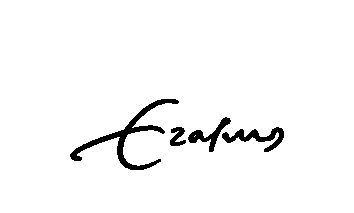
\includegraphics[height=9em]{./logos/EUR_signature_02_RGB_black}
\end{center}

% ************************************************************************

\newpage
\thispagestyle{empty}
\label{othersideformal}

\begin{tabular}{@{}ll@{}}
\large\bf{Promotiecommissie} &\\ [8ex]
Promotor:      & {\bf Prof.dr.~W.J.~Niessen}\\[3ex]
Overige leden: & {\bf Prof.dr.ir.~P.H.E.~Tiesinga}\\[1ex]
               & {\bf Prof.dr.ir.~F.J.~Verbeek}\\[1ex]
               & {\bf Prof.dr.~C.I.~de Zeeuw}\\[3ex]
Copromotor:    & {\bf Dr.ir.~H.W.~Meijering}\\
\end{tabular}
